\subsection{Qualità di processo standard ISO/IEC 15504}\label{15504}
Lo standard ISO/IEC 15504 descrive come i processi debbano essere continuamente controllati in modo da rilevare possibili rischi e debolezze che possano impedire il raggiungimento degli scopi prefissati e di individuarne le cause in modo di migliore l'efficienza dei processi. I risultati dei vari controlli devono essere oggettivi, ripetibili e comparabili perché possano essere utilizzati nel miglioramento dei processi.

\noindent Lo standard ISO/IEC 15504, conosciuto anche come SPICE(Software Process Improvement and Capability Determination), prevede per ogni processo un livello di capacità secondo la seguente ripartizione:

\begin{enumerate}[label*=\arabic*]
	\item \textbf{Incomplete process:} il processo non viene eseguito o non riesce a raggiungere i suoi risultati;
	
	\item \textbf{Performed:} il processo eseguito raggiunge i suoi risultati
		\begin{itemize}
			\item \textbf{Process performance attribute:} è la capacità di un processo di raggiungere gli obiettivi trasformando input identificabili in output identificabili.
		\end{itemize}
		
	\item \textbf{Managed process:} il processo viene eseguito in modo controllato in base a obiettivi definiti
		\begin{itemize}
			\item \textbf{Performance management attribute:} è la capacità del processo di elaborare un prodotto coerente con gli obiettivi fissati;
			\item \textbf{Work product management attribute:} è la capacità del processo di elaborare un prodotto documentato, controllato e verificato.
		\end{itemize}
		
		
	\item \textbf{Established process:} il processo viene eseguito basandosi su principi dell'ingegneria del software ed è in grado di raggiungere i risultati fissati
		\begin{itemize}
			\item \textbf{Process definition attribute:} l'esecuzione del processo si basa su standard di processo per raggiungere i propri obiettivi;
			\item \textbf{Process resource attribute:} è la capacità del processo di attingere a risorse tecniche e umane appropriate per essere attuato efficacemente.
		\end{itemize}
		
	\item \textbf{Predictable process:} il processo viene eseguito costantemente entro limiti definiti per raggiungere i risultati attesi
		\begin{itemize}
			\item\textbf{Measurement attribute:} sono gli obiettivi e le misure di prodotto e di processo che vengono usati per garantire il raggiungimento dei traguardi definiti in supporto ai target aziendali;
			\item \textbf{Process control attribute:} il processo viene controllato tramite misure di prodotto e processo per effettuare correzioni migliorative al processo stesso.
		\end{itemize}
		
\item \textbf{Optimizing process:} il processo cambia e si adatta dinamicamente per raggiungere gli obiettivi aziendali
		\begin{itemize}
			\item \textbf{Process change attribute:} sono i cambiamenti strutturali, di gestione e di esecuzione che vengono gestiti in modo controllato per raggiungere i risultati fissati;
			\item \textbf{Continuous improvement attribute:} sono le modifiche al processo che sono identificate e implementate per garantire il miglioramento continuo nella realizzazione degli obiettivi di \gls{business} dell'organizzazione.
		\end{itemize}

\end{enumerate}

\noindent Ogni attributo di processo descritto sopra è misurabile e lo standard predispone 4 livelli diversi:
\begin{itemize}[label={}]
	\item \textbf{N} non posseduto (0\% - 15\%);
	\item \textbf{P} parzialmente posseduto (16\% - 50\%);
	\item \textbf{L} largamente posseduto (51\% - 85\%);
	\item \textbf{F} completamente posseduto (86\% - 100\%).
\end{itemize}

\subsection{Qualità di prodotto standard ISO/IEC 9126} \label{9126}
Con la sigla \textbf{ISO/IEC 9126} s'individua una serie di normative e linee guida preposte a descrivere un modello di qualità del software.
Esso divide i criteri qualitativi in 3 aree diverse:
\begin{itemize}

	\item \textbf{Qualità in uso:} rappresenta il punto di vista dell'utente sul software;
	\item \textbf{Qualità esterna:} misurano i comportamenti del software sulla base dei test, dall'operatività e dall'osservazione durante la sua esecuzione;
	\item \textbf{Qualità interna:} è la qualità del prodotto software vista dall'interno, si riferisce quindi alle caratteristiche d'implementazione quali l'architettura ed i codici sorgenti.
\end{itemize}

\noindent Il modello di qualità dello standard prevede 6 caratteristiche qualitative principali, suddivise in ulteriori sotto caratteristiche, misurabili quantitativamente tramite metriche specifiche.

\begin{figure}[h]
\centering
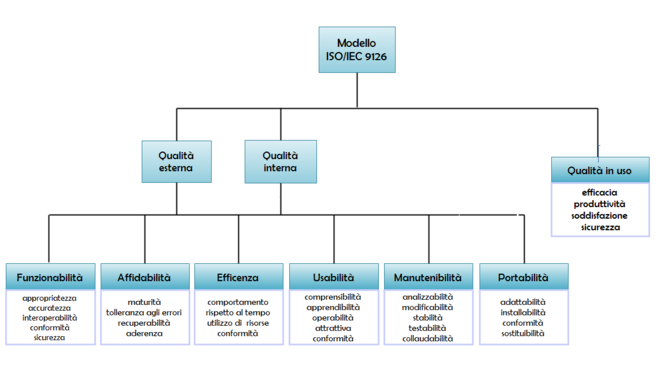
\includegraphics[width=0.7\linewidth]{img/ISO_IEC_9126}
\caption[Rappresentazione globale del modello ISO-IEC 9126]{Rappresentazione globale del modello ISO-IEC 9126}
\label{fig:ISO_IEC_9126}
\end{figure}


\begin{itemize}
\item \textbf{Funzionalità:} è la capacità di un prodotto software di fornire funzioni che soddisfano esigenze stabilite:

\begin{itemize}
	\item \textbf{Idoneità:}  rappresenta la capacità del prodotto software di fornire un appropriato insieme di funzioni per gli specificati compiti e obiettivi prefissati all'utente;
	\item \textbf{Accuratezza:} è la capacità del prodotto software di fornire i risultati concordati;
	\item \textbf{Interoperabilità:} è la capacità del prodotto software di interagire ed operare con uno o più sistemi;
	\item \textbf{Conformità:} è la capacità del prodotto software di aderire a standard, convenzioni e regolamentazioni;
	\item \textbf{Sicurezza:} è la capacità del prodotto software di proteggere informazioni e dati impedendo che persone o sistemi non autorizzati passano accedervi o modificarli.
\end{itemize}

\item \textbf{Affidabilità:} è la capacità del prodotto software di mantenere uno specificato livello di prestazioni:
\begin{itemize}
	\item \textbf{Maturità:} è la capacità di un prodotto software di evitare che si verificano errori o malfunzionamenti;
	\item \textbf{Tolleranza agli errori:} è la capacità di un prodotto software di mantenere un adeguato livello di prestazioni anche nel caso si verifichino errore o malfunzionamenti;
	\item \textbf{Recuperabilità:} è la capacità del prodotto software di ristabilire un adeguato livello di performance e di recuperare i dati interessati in caso di errori;
	\item \textbf{Aderenza:} è la capacità di aderire a standard, regole e convenzioni inerenti all'affidabilità.
\end{itemize}

\item \textbf{Efficienza:} è la capacità di fornire appropriate prestazioni relativamente alla quantità di risorse usate:
\begin{itemize}
	\item \textbf{Comportamento rispetto al tempo:} è la capacità di fornire adeguati tempi di risposta, elaborazione e velocità sotto determinate condizioni;
	\item \textbf{Utilizzo delle risorse:} è la capacità di utilizzo di quantità e tipo di risorse in maniera adeguata;
	\item \textbf{Conformità:} è la capacità di aderire a standard e specifiche sull'efficienza.
\end{itemize}

\item \textbf{Usabilità:} è la capacità del prodotto software di essere appreso e usato dall'utente sotto specifiche condizioni:
\begin{itemize}
	\item \textbf{Comprensibilità:} esprime la facilità di comprensione dei concetti del prodotto;
	\item \textbf{Apprendibilità:} è la capacità di ridurre l'impegno richiesto agli utenti per apprendere l'uso del prodotto;
	\item \textbf{Operabilità:} è la capacità del prodotto software di consentire all'utente di usarlo e controllarlo;
	\item \textbf{Attrattività:} è la capacità del software di essere piacevole per l'utente che ne fa uso;
	\item \textbf{Conformità:} è la capacità del software di aderire a standard o convenzioni relativi l'usabilità.
\end{itemize}
\item \textbf{Manutenibilità:} è la capacità del software di essere modificato, includendo correzioni, miglioramenti o adattamenti:
\begin{itemize}
	\item \textbf{Analizzabilità:} rappresenta la facilità con la quale è possibile analizzare il codice per localizzare un errore;
	\item \textbf{Modificabilità:} è la capacità del prodotto software di permettere l'implementazione di una specificata modifica;
	\item \textbf{Stabilità:} è la capacità del software di evitare effetti inaspettati derivanti da modifiche errate;
	\item \textbf{Testabilità:} è la capacità di essere facilmente testato per validare le modifiche apportate al software.
\end{itemize}

\item \textbf{Portabilità:} è la capacità del software di essere trasportato da un ambiente di lavoro a un altro:
\begin{itemize}
	\item \textbf{Adattabilità:} è la capacità del software di essere adattato per differenti ambienti operativi senza dover applicare modifiche;
	\item \textbf{Installabilità:} è la capacità del software di essere installato in uno specificato ambiente;
	\item \textbf{Conformità:} è la capacità del prodotto software di aderire a standard e convenzioni relative la portabilità;
	\item \textbf{Sostituibilità:} è la capacità di essere utilizzato al posto di un altro software per svolgere gli stessi compiti nello stesso ambiente.
\end{itemize}

\end{itemize}


\subsection{Metriche per i processi}
\label{sezione 3.7}
Per misurare lo stato di avanzamento dei processi si è scelto di utilizzare indici che ne analizzino i costi e
tempi.
\subsubsection{Schedule Variance (SV)}
Lo Schedule Variance è un indicatore di efficacia e serve a controllare se si è in linea, in anticipo o in ritardo rispetto alla pianificazione temporale delle attività nella baseline.
Se SV G > 0 significa che il gruppo di lavoro sta producendo con maggior velocità rispetto a quanto pianificato, viceversa se negativo.
Essendo stati inseriti slack durante la pianificazione della baseline dei processi, il valore di tale indice è inizialmente positivo.
Parametri utilizzati:
\begin{itemize}
	\item \textbf{Range-accettazione}: $\left[  \geq - \: costo \: preventivo \: fase * 5 \% \right]$
	\item \textbf{Range-ottimale}: $\left[\geq 0\right]$.
\end{itemize}
\subsubsection{Budget Variance (BV)}
Il Budget Variance è un indicatore che ha un valore contabile e finanziario e che serve a controllare se alla data corrente si è speso di più o di meno rispetto a quanto pianificato.
Se BV G > 0 significa che l'attuazione del progetto sta consumando il proprio budget con minor velocità rispetto a quanto pianificato, viceversa se negativo.
Parametri utilizzati:
\begin{itemize}
	\item \textbf{Range-accettazione}: $\left[  \geq - \: costo \: preventivo \: fase * 10 \% \right]$
	\item \textbf{Range-ottimale}: $\left[\geq 0\right]$.
\end{itemize}

\subsection{Metriche per la documentazione}
\label{sezione 3.8}
Come metrica per i documenti redatti si è deciso di utilizzare l'indice di leggibilità Gulpease. Rispetto ad altri ha il vantaggio di utilizzare la lunghezza delle parole in lettere anziché in sillabe, semplificandone il calcolo automatico. L'indice è tarato sulla lingua italiana e considera due variabili linguistiche: la lunghezza della parola e la lunghezza della frase rispetto al numero delle lettere. \\
\noindent L'indice è calcolato attraverso la seguente formula:\\
\begin{center}
	$89+ \frac{300*\left(numero\:\ delle\:\ frasi \right)-10*\left(numero\:\ delle\:\ lettere\right)}{numero\:\ delle\:\ parole}$
\end{center}
I risultati sono compresi tra 0 e 100, dove 100 indica la leggibilità più alta e 0 la leggibilità più bassa. In generale risulta che i testi con indice:
\begin{itemize}
	\item Inferiore a 80 sono difficili da leggere per chi ha la licenza elementare;
	\item Inferiore a 60 sono difficili da leggere per chi ha la licenza media;
	\item Inferiore a 40 sono difficile da leggere per chi ha il diploma superiore.
\end{itemize}
Basandoci su queste considerazioni è stato scelto di utilizzare:
\begin{itemize}
	\item \textbf{Range di accettazione:} [40 - 100];
	\item \textbf{Range ottimale:} [50 - 100].
\end{itemize}
	
\subsection{Metriche per il software}
Di seguito saranno descritte le metriche che riguardano il software. Data l'inesperienza del gruppo, questa sezione sarà soggetta a modifiche nelle prossime revisioni.
\begin{itemize}
	\item \textbf{Complessità ciclomatica:} misura direttamente il numero di cammini linearmente indipendenti attraverso il grafo di controllo di flusso. Essa viene calcolata utilizzando il grafo di controllo di flusso del programma: i nodi del grafo corrispondono a gruppi indivisibili di istruzioni, mentre gli archi connettono due nodi se il secondo gruppo di istruzioni può essere eseguito immediatamente dopo il primo gruppo. La complessità ciclomatica può, inoltre, essere applicata a singole funzioni, moduli, metodi o classi di un programma.
	\begin{itemize}
		\item \textbf{Range di accettazione:} [1 - 15];
		\item \textbf{Range ottimale:} [1 - 10].
	\end{itemize}
	\item \textbf{Attributi per classe:} un numero elevato di attributi all'interno della classe potrebbe indicare il bisogno di suddividere la classe in più sotto classi.
	\begin{itemize}
		\item \textbf{Range di accettazione:} [0 - 16];
		\item \textbf{Range ottimale:} [3 - 8].
	\end{itemize}
	\item \textbf{Numero di parametri per metodo:} indica il numero di parametri formali di un metodo. Un numero elevato di parametri potrebbe indicare la necessità di ridurre le funzionalità associate a tale metodo.
	\begin{itemize}
		\item \textbf{Range di accettazione:} [0 - 8];
		\item \textbf{Range ottimale:} [0 - 4].
	\end{itemize}
	\item \textbf{Linee di codice per linee di commento:} indica il rapporto tra il numero di linee di commento e il numero di linee di codice. Il codice poco commentato comporta una difficile manutenibilità.
	\begin{itemize}
		\item \textbf{Range di accettazione:} [>20];
		\item \textbf{Range ottimale:} [>30].
	\end{itemize}
	\item \textbf{Numero di livelli di annidamento:} indica il numero di livelli di annidamento dei metodi. Un numero elevato rappresenta un'alta complessità del codice riducendone il livello di astrazione.
	\begin{itemize}
		\item \textbf{Range di accettazione:} [1 - 6];
		\item \textbf{Range ottimale:} [1 - 3].
	\end{itemize}
	\item \textbf{Copertura del codice:} valore che indica la percentuale di codice che viene eseguito durante i test.
	Un valore elevato indica un'alta probabilità che i moduli testati abbiano pochi errori.
	\begin{itemize}
		\item \textbf{Range di accettazione:} [ $\geq$ 40\%];
		\item \textbf{Range ottimale:} [ $\geq$ 60\%].
	\end{itemize}
\end{itemize}



